\documentclass[addpoints]{exam}
\usepackage[utf8]{inputenc}
\usepackage{multicol}
\usepackage{graphicx}
\usepackage{amsmath}
\usepackage[a4paper,top=15mm, bottom=15mm, left=15mm, right=15mm]{geometry}
 
\begin{document}
	
	Dal seguente diagramma ER proposto, crea il corrispondente schema logico come visto nelle scorse lezioni e svolgi le seguenti azioni usando il codice SQL:
	\begin{itemize}
		\item Crea le tabelle Sezione, Ricercatore e Progetto
		\item Inserisci un valore (decidi tu i dati) nella tabella Ricercatore
		\item Visualizza il responsabile della sezione "Informatica"
		\item Visualizza i ricercatori della sezione "Filosofia"
		\item Visualizza le sezioni che hanno come obiettivo "Algoritmi innovativi"
	\end{itemize}

	\begin{figure}[h!]
		\centering
		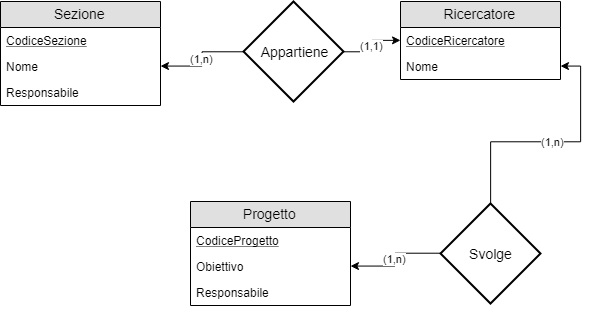
\includegraphics[scale=0.5]{images/Ricercatori.png}
	\end{figure}

	\vspace{40mm}
	
	Dal seguente diagramma ER proposto, crea il corrispondente schema logico come visto nelle scorse lezioni e svolgi le seguenti azioni usando il codice SQL:
	\begin{itemize}
		\item Crea le tabelle Sezione, Ricercatore e Progetto
		\item Inserisci un valore (decidi tu i dati) nella tabella Ricercatore
		\item Visualizza il responsabile della sezione "Informatica"
		\item Visualizza i ricercatori della sezione "Filosofia"
		\item Visualizza le sezioni che hanno come obiettivo "Algoritmi innovativi"
	\end{itemize}
	
	\begin{figure}[h!]
		\centering
		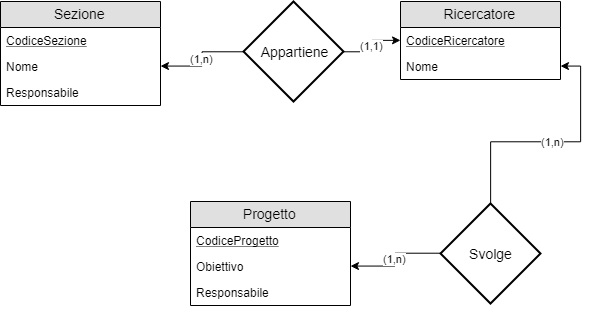
\includegraphics[scale=0.5]{images/Ricercatori.png}
	\end{figure}
\end{document}